% ============================================================
% Question Bank: ch02-01 Solving Percent Problems
% Topic Title: Solving Percent Problems
% CCSS: 7.RP.A.3
% Questions: 27 (15 MC + 6 SA + 6 Graphical)
% ============================================================

% --- Multiple Choice Questions (15) ---

\begin{practiceQuestion}{2-1-q01}{mc}
\begin{questionText}
A pet shelter has $120$ animals. If $45\%$ are cats, how many cats are in the shelter?
\end{questionText}
\choiceA{$45$}
\choiceB{$54$}
\choiceC{$60$}
\choiceD{$75$}
\correctAnswer{B}
\explanation{Convert the percent to a decimal: $45\% = 0.45$. Multiply by the whole: $0.45 \times 120 = 54$ cats.}
\end{practiceQuestion}

\begin{practiceQuestion}{2-1-q02}{mc}
\begin{questionText}
$28$ is what percent of $112$?
\end{questionText}
\choiceA{$4\%$}
\choiceB{$20\%$}
\choiceC{$25\%$}
\choiceD{$28\%$}
\correctAnswer{C}
\explanation{Divide the part by the whole: $28 \div 112 = 0.25$. Convert to a percent: $0.25 \times 100 = 25\%$.}
\end{practiceQuestion}

\begin{practiceQuestion}{2-1-q03}{mc}
\begin{questionText}
$72$ is $90\%$ of what number?
\end{questionText}
\choiceA{$64.8$}
\choiceB{$75$}
\choiceC{$78$}
\choiceD{$80$}
\correctAnswer{D}
\explanation{Divide the part by the percent: $72 \div 0.90 = 80$. The whole is $80$.}
\end{practiceQuestion}

\begin{practiceQuestion}{2-1-q04}{mc}
\begin{questionText}
During a fundraiser, a school collected $\$840$ out of its $\$1{,}200$ goal. What percent of the goal has been reached?
\end{questionText}
\choiceA{$60\%$}
\choiceB{$65\%$}
\choiceC{$70\%$}
\choiceD{$84\%$}
\correctAnswer{C}
\explanation{Divide the part by the whole: $840 \div 1{,}200 = 0.70$. Multiply by $100$: the school has reached $70\%$ of its goal.}
\end{practiceQuestion}

\begin{practiceQuestion}{2-1-q05}{mc}
\begin{questionText}
What is $175\%$ of $60$?
\end{questionText}
\choiceA{$75$}
\choiceB{$95$}
\choiceC{$105$}
\choiceD{$120$}
\correctAnswer{C}
\explanation{Convert: $175\% = 1.75$. Multiply: $1.75 \times 60 = 105$. A percent greater than $100\%$ gives a result greater than the whole.}
\end{practiceQuestion}

\begin{practiceQuestion}{2-1-q06}{mc}
\begin{questionText}
A factory inspected $350$ parts and found that $14$ were defective. What percent of the parts were defective?
\end{questionText}
\choiceA{$2\%$}
\choiceB{$4\%$}
\choiceC{$5\%$}
\choiceD{$14\%$}
\correctAnswer{B}
\explanation{Divide: $14 \div 350 = 0.04$. Multiply by $100$: $4\%$ of the parts were defective.}
\end{practiceQuestion}

\begin{practiceQuestion}{2-1-q07}{mc}
\begin{questionText}
$48$ is $60\%$ of what number?
\end{questionText}
\choiceA{$28.8$}
\choiceB{$72$}
\choiceC{$80$}
\choiceD{$108$}
\correctAnswer{C}
\explanation{Divide the part by the percent: $48 \div 0.60 = 80$. Check: $0.60 \times 80 = 48$ \checkmark.}
\end{practiceQuestion}

\begin{practiceQuestion}{2-1-q08}{mc}
\begin{questionText}
A gym has $160$ members. If $35\%$ attend on Monday, how many members attend?
\end{questionText}
\choiceA{$35$}
\choiceB{$52$}
\choiceC{$56$}
\choiceD{$64$}
\correctAnswer{C}
\explanation{Convert: $35\% = 0.35$. Multiply: $0.35 \times 160 = 56$ members attend on Monday.}
\end{practiceQuestion}

\begin{practiceQuestion}{2-1-q09}{mc}
\begin{questionText}
A student scored $78$ out of $120$ points on a project. What percent did the student earn?
\end{questionText}
\choiceA{$55\%$}
\choiceB{$60\%$}
\choiceC{$65\%$}
\choiceD{$78\%$}
\correctAnswer{C}
\explanation{Divide the part by the whole: $78 \div 120 = 0.65$. Convert: $0.65 \times 100 = 65\%$.}
\end{practiceQuestion}

\begin{practiceQuestion}{2-1-q10}{mc}
\begin{questionText}
Which proportion can be used to find what number is $55\%$ of $260$?
\end{questionText}
\choiceA{$\dfrac{n}{260} = \dfrac{55}{100}$}
\choiceB{$\dfrac{260}{n} = \dfrac{55}{100}$}
\choiceC{$\dfrac{55}{260} = \dfrac{n}{100}$}
\choiceD{$\dfrac{n}{55} = \dfrac{260}{100}$}
\correctAnswer{A}
\explanation{The part $n$ is over the whole $260$, and the percent $55$ is over $100$: $\frac{n}{260} = \frac{55}{100}$.}
\end{practiceQuestion}

\begin{practiceQuestion}{2-1-q11}{mc}
\begin{questionText}
A community garden has $75$ plots. If $60\%$ are growing vegetables and the rest grow flowers, how many grow flowers?
\end{questionText}
\choiceA{$25$}
\choiceB{$30$}
\choiceC{$40$}
\choiceD{$45$}
\correctAnswer{B}
\explanation{Flowers are $100\% - 60\% = 40\%$ of the plots. Multiply: $0.40 \times 75 = 30$ plots grow flowers.}
\end{practiceQuestion}

\begin{practiceQuestion}{2-1-q12}{mc}
\begin{questionText}
$0.5\%$ of $1{,}600$ is what number?
\end{questionText}
\choiceA{$0.8$}
\choiceB{$8$}
\choiceC{$80$}
\choiceD{$800$}
\correctAnswer{B}
\explanation{Convert: $0.5\% = 0.005$. Multiply: $0.005 \times 1{,}600 = 8$. Be careful — $0.5\%$ is much smaller than $5\%$.}
\end{practiceQuestion}

\begin{practiceQuestion}{2-1-q13}{mc}
\begin{questionText}
A water tank holds $400$ gallons. It is $82\%$ full. How many gallons of water are in the tank?
\end{questionText}
\choiceA{$318$}
\choiceB{$320$}
\choiceC{$328$}
\choiceD{$340$}
\correctAnswer{C}
\explanation{Convert: $82\% = 0.82$. Multiply: $0.82 \times 400 = 328$ gallons.}
\end{practiceQuestion}

\begin{practiceQuestion}{2-1-q14}{mc}
\begin{questionText}
$51$ is $\frac{1}{3}\%$ of what number? (Hint: $\frac{1}{3}\% \approx 0.333\%$.)
\end{questionText}
\choiceA{$153$}
\choiceB{$1{,}530$}
\choiceC{$15{,}300$}
\choiceD{$51{,}000$}
\correctAnswer{C}
\explanation{Convert: $\frac{1}{3}\% = \frac{1}{300}$. Divide: $51 \div \frac{1}{300} = 51 \times 300 = 15{,}300$. This is the whole.}
\end{practiceQuestion}

\begin{practiceQuestion}{2-1-q15}{mc}
\begin{questionText}
On a test, Malik answered $39$ out of $52$ questions correctly. His teacher said he got $75\%$ correct. Is the teacher right?
\end{questionText}
\choiceA{Yes, $39 \div 52 = 0.75$}
\choiceB{No, the correct percent is $70\%$}
\choiceC{No, the correct percent is $65\%$}
\choiceD{No, the correct percent is $80\%$}
\correctAnswer{A}
\explanation{Divide the part by the whole: $39 \div 52 = 0.75 = 75\%$. The teacher is correct.}
\end{practiceQuestion}

% --- Short Answer Questions (6) ---

\begin{practiceQuestion}{2-1-q16}{sa}
\begin{questionText}
A bookstore has $450$ books. If $36\%$ are paperback, how many paperback books are there?
\end{questionText}
\correctAnswer{$162$}
\explanation{Convert the percent: $36\% = 0.36$. Multiply: $0.36 \times 450 = 162$ paperback books.}
\end{practiceQuestion}

\begin{practiceQuestion}{2-1-q17}{sa}
\begin{questionText}
$63$ is what percent of $84$?
\end{questionText}
\correctAnswer{$75\%$}
\explanation{Divide the part by the whole: $63 \div 84 = 0.75$. Convert: $0.75 \times 100 = 75\%$.}
\end{practiceQuestion}

\begin{practiceQuestion}{2-1-q18}{sa}
\begin{questionText}
A survey shows that $92\%$ of $225$ students have a smartphone. How many students have a smartphone?
\end{questionText}
\correctAnswer{$207$}
\explanation{Convert: $92\% = 0.92$. Multiply: $0.92 \times 225 = 207$ students.}
\end{practiceQuestion}

\begin{practiceQuestion}{2-1-q19}{sa}
\begin{questionText}
$84$ is $140\%$ of what number?
\end{questionText}
\correctAnswer{$60$}
\explanation{Divide the part by the percent: $84 \div 1.40 = 60$. A percent greater than $100\%$ means the part is larger than the whole.}
\end{practiceQuestion}

\begin{practiceQuestion}{2-1-q20}{sa}
\begin{questionText}
A recipe uses $180$ grams of flour out of $720$ grams of total ingredients. What percent is flour?
\end{questionText}
\correctAnswer{$25\%$}
\explanation{Divide the part by the whole: $180 \div 720 = 0.25$. Multiply by $100$: flour is $25\%$ of the total.}
\end{practiceQuestion}

\begin{practiceQuestion}{2-1-q21}{sa}
\begin{questionText}
A charity wants to raise $\$5{,}000$. So far they have $\$3{,}750$. What percent of the goal have they reached?
\end{questionText}
\correctAnswer{$75\%$}
\explanation{Divide by the goal: $3{,}750 \div 5{,}000 = 0.75$. Convert: $0.75 \times 100 = 75\%$ of the goal.}
\end{practiceQuestion}

% --- Graphical Questions (3 GMC + 3 GSA) ---

\begin{practiceQuestion}{2-1-q22}{gmc}
\begin{questionText}
The $10 \times 10$ grid below has some squares shaded. What percent of the grid is \textbf{not} shaded?

\begin{center}
\begin{tikzpicture}[scale=0.35]
  \foreach \x in {0,...,9} {
    \foreach \y in {0,...,9} {
      \draw[gray!50] (\x,\y) rectangle (\x+1,\y+1);
    }
  }
  % Shade 42 squares (rows 0-3 full = 40, plus 2 in row 4)
  \foreach \x in {0,...,9} {
    \foreach \y in {0,...,3} {
      \fill[funOrange!40] (\x,\y) rectangle (\x+1,\y+1);
      \draw[gray!50] (\x,\y) rectangle (\x+1,\y+1);
    }
  }
  \foreach \x in {0,...,1} {
    \fill[funOrange!40] (\x,4) rectangle (\x+1,5);
    \draw[gray!50] (\x,4) rectangle (\x+1,5);
  }
\end{tikzpicture}
\end{center}
\end{questionText}
\choiceA{$42\%$}
\choiceB{$48\%$}
\choiceC{$55\%$}
\choiceD{$58\%$}
\correctAnswer{D}
\explanation{The grid has $100$ squares. Shaded: $4$ full rows of $10 = 40$, plus $2$ more $= 42$. Not shaded: $100 - 42 = 58$. So $58\%$ is not shaded.}
\end{practiceQuestion}

\begin{practiceQuestion}{2-1-q23}{gmc}
\begin{questionText}
The table shows the results of a class vote for a class pet. What percent of the class voted for a hamster?

\begin{center}
\begin{tabular}{|l|c|}
\hline
\textbf{Pet} & \textbf{Votes} \\
\hline
Fish & $8$ \\
\hline
Hamster & $12$ \\
\hline
Turtle & $5$ \\
\hline
Rabbit & $5$ \\
\hline
\end{tabular}
\end{center}
\end{questionText}
\choiceA{$12\%$}
\choiceB{$30\%$}
\choiceC{$40\%$}
\choiceD{$48\%$}
\correctAnswer{C}
\explanation{Total votes: $8 + 12 + 5 + 5 = 30$. Hamster percent: $12 \div 30 = 0.40 = 40\%$.}
\end{practiceQuestion}

\begin{practiceQuestion}{2-1-q24}{gmc}
\begin{questionText}
The tape diagram below represents a whole quantity of $90$. What percent does the shaded section represent?

\begin{center}
\begin{tikzpicture}[scale=0.65]
  \foreach \i in {0,...,5} {
    \draw[thick] (\i*1.4,0) rectangle (\i*1.4+1.4,0.8);
  }
  \fill[funBlue!40] (0,0) rectangle (1.4,0.8);
  \fill[funBlue!40] (1.4,0) rectangle (2.8,0.8);
  \foreach \i in {0,...,5} {
    \draw[thick] (\i*1.4,0) rectangle (\i*1.4+1.4,0.8);
  }
  \node[below,font=\small] at (0.7,0) {$15$};
  \node[below,font=\small] at (2.1,0) {$15$};
  \node[below,font=\small] at (3.5,0) {$15$};
  \node[below,font=\small] at (4.9,0) {$15$};
  \node[below,font=\small] at (6.3,0) {$15$};
  \node[below,font=\small] at (7.7,0) {$15$};
  \draw[thick,<->] (0,-0.9) -- (8.4,-0.9) node[midway,below,font=\small] {Total $= 90$};
\end{tikzpicture}
\end{center}
\end{questionText}
\choiceA{$15\%$}
\choiceB{$20\%$}
\choiceC{$30\%$}
\choiceD{$\tfrac{100}{3}\%$}
\correctAnswer{D}
\explanation{Two out of six equal sections are shaded. The shaded part is $\frac{2}{6} = \frac{1}{3}$ of the whole. As a percent: $\frac{1}{3} \times 100 = 33.\overline{3}\%$, or $\frac{100}{3}\%$.}
\end{practiceQuestion}

\begin{practiceQuestion}{2-1-q25}{gsa}
\begin{questionText}
The bar graph below shows the number of books read by four students in one month. What percent of the total books were read by Zoe?

\begin{center}
\begin{tikzpicture}[scale=0.5]
  \draw[thick,->] (0,0) -- (0,7) node[above]{\small Books};
  \draw[thick,->] (0,0) -- (9,0);
  \fill[funBlue!60] (0.5,0) rectangle (1.5,4);
  \fill[funGreen!60] (2.5,0) rectangle (3.5,6);
  \fill[funOrange!60] (4.5,0) rectangle (5.5,5);
  \fill[funRed!60] (6.5,0) rectangle (7.5,5);
  \node[below,font=\small] at (1,0) {Ava};
  \node[below,font=\small] at (3,0) {Zoe};
  \node[below,font=\small] at (5,0) {Leo};
  \node[below,font=\small] at (7,0) {Mia};
  \foreach \y/\lab in {1/2,2/4,3/6,4/8,5/10,6/12} {
    \draw (-0.1,\y) -- (0.1,\y) node[left,font=\small,xshift=-2pt] {\lab};
  }
  \node[above,font=\small] at (1,4) {$8$};
  \node[above,font=\small] at (3,6) {$12$};
  \node[above,font=\small] at (5,5) {$10$};
  \node[above,font=\small] at (7,5) {$10$};
\end{tikzpicture}
\end{center}
\end{questionText}
\correctAnswer{$30\%$}
\explanation{Total books: $8 + 12 + 10 + 10 = 40$. Zoe read $12$. Percent: $12 \div 40 = 0.30 = 30\%$.}
\end{practiceQuestion}

\begin{practiceQuestion}{2-1-q26}{gsa}
\begin{questionText}
The circle graph below shows how a student spends $20$ hours each week on activities. How many hours does the student spend on homework?

\begin{center}
\begin{tikzpicture}[scale=1.7]
  % Pie chart: Sports 30%, Homework 25%, Video games 20%, Reading 25%
  \fill[funBlue!50] (0,0) -- (90:1) arc (90:198:1) -- cycle;
  \fill[funGreen!50] (0,0) -- (198:1) arc (198:270:1) -- cycle;
  \fill[funOrange!50] (0,0) -- (270:1) arc (270:360:1) -- cycle;
  \fill[funRed!50] (0,0) -- (0:1) arc (0:90:1) -- cycle;
  \draw (0,0) circle (1);
  \draw (0,0) -- (90:1); \draw (0,0) -- (198:1);
  \draw (0,0) -- (270:1); \draw (0,0) -- (0:1);
  \node[font=\small, align=center] at (144:0.6) {Sports\\$30\%$};
  \node[font=\small, align=center] at (234:0.6) {Games\\$20\%$};
  \node[font=\small, align=center] at (315:0.6) {Reading\\$25\%$};
  \node[font=\small, align=center] at (45:0.6) {HW\\$25\%$};
\end{tikzpicture}
\end{center}
\end{questionText}
\correctAnswer{$5$ hours}
\explanation{Homework is $25\%$ of the $20$ hours. Multiply: $0.25 \times 20 = 5$ hours on homework.}
\end{practiceQuestion}

\begin{practiceQuestion}{2-1-q27}{gsa}
\begin{questionText}
The double number line below shows the relationship between a number and its percent. What value belongs at the question mark?

\begin{center}
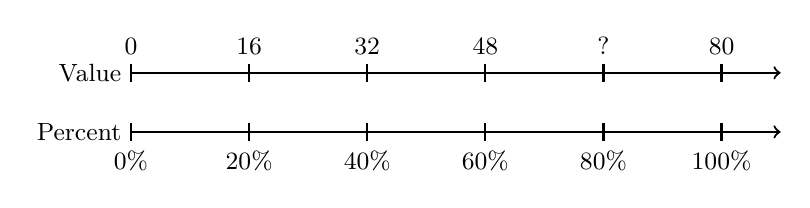
\begin{tikzpicture}[scale=0.75]
  \draw[thick,->] (0,1) -- (11,1);
  \node[left,font=\small] at (0,1) {Value};
  \foreach \x/\lab in {0/0, 2/16, 4/32, 6/48, 8/?, 10/80} {
    \draw[thick] (\x,0.85) -- (\x,1.15);
    \node[above,font=\small] at (\x,1.15) {\lab};
  }
  \draw[thick,->] (0,0) -- (11,0);
  \node[left,font=\small] at (0,0) {Percent};
  \foreach \x/\lab in {0/0\%, 2/20\%, 4/40\%, 6/60\%, 8/80\%, 10/100\%} {
    \draw[thick] (\x,-0.15) -- (\x,0.15);
    \node[below,font=\small] at (\x,-0.15) {\lab};
  }
\end{tikzpicture}
\end{center}
\end{questionText}
\correctAnswer{$64$}
\explanation{The whole ($100\%$) is $80$. The question mark is at $80\%$. Multiply: $0.80 \times 80 = 64$.}
\end{practiceQuestion}
